\chapter{Introduction\label{cha:introduction}}
%% \ifdraft only shows the text in the first argument if you are in draft mode.
%% These directions will disappear in other modes.

% \ifdraft{State the objectives of the exercise. Ask yourself:
%   \underline{Why} did I design/create the item? What did I aim to
%   achieve? What is the problem I am trying to solve?  How is my
%   solution interesting or novel?}{}

% The object of the project is to be able to monitor cetacean traffic around Iceland.
% This could help tourism companies relating to whale watching. 
% Could also be extended to whale researchers.


Humans have caused increased pressure on animals whether that be land or sea creatures.
Keeping track of the creatures is vital to ensure their health and survival for the future.
This can be done by population assessments, which can show if the specific species is in an upsurge or declining in terms of numbers.
For fish and cetaceans, there are several ways to achieve this for example the animal can be tracked via Global Positioning System (GPS) tracker or the animal is visually sighted by the use of a boat or aircraft.
These methods are however time consuming and require a lot of man power.
To plant a tracker on the animal it must first be found and captured in order to attach the tracker and the later method requires researchers to actively search the animal, which is heavily reliant on favourable sea conditions etc.
There is however methods available that rely on acoustic surveys in order to monitor cetaceans which enables researchers to not only explore the surface of the ocean but also beneath the waves.
These surveys can be done in several ways.
One method involves dragging an array of hydrophones and record the vocalization data.
The second is to mount hydrophones into the bow of the ship and record the vocalization data.
These method however can not be used when recording low frequency sounds, due to noise created by the ship and water flow as well as still requiring researchers on board ships actively looking for animals.
The third method, and the one this thesis will focus on is a passive buoy sound gathering.
Where a hydrophone and a recording device are attached to a buoy that moored in place and sets on recording passively that location without the need of external help and maintenance.

The buoy must be self sufficient and able to stay out at sea for long periods at a time to serve its function.
This means that all the electronics on board will need to be powered by the buoy.
It also has to be able to record cetacean vocalization and transmit the data onshore.
So that marine researchers can study the data or even whale watching companies in the tourism industry can play cetacean vocalizations in the fjords.
This means the passive sound gathering buoy can be separated into three different projects, power production, sound gathering and data transmission onshore.
This thesis will focus on developing a device for the cetacean vocalization recording.

This function will be implemented using a Teensy 3.5 microcontroller.
A hydrophone will be used in order to sense the sound waves generated by the cetacean vocalization which have an extremely wide frequency range of a few Hz all the way to echolocation signals which are hundreds of thousands of Hz, this project will have therefore gather signals in the range of 10Hz to 100kHz, at at least 16bits resolution for high quality audio.
The electrical circuit will consist of a preamplifier, filter, analog to digital converter and SD card for data logging.
The circuit will refine the signal to be readable for the microcontroller. 


\section{Project Goals}

The objective of the project is to create a relatively small, low cost and low maintenance device capable of recording cetacean vocalization and transmitting the data onshore.
The design criteria for the project is as follows.
The total power consumption to the system should be less than 10 watts. 
The device should be relatively small and lightweight,so it is deployable by one person.
The device should last 6 months at a time.
Be able to gather data of signal ranging from 10Hz to 100kHz.
\clearpage

\section{Background}

Considerable cetacean preservation efforts have been carried out for the past decades.
In 1946 the International whale commission, which is a global body with the goal of conservation of whales and currently has 88 member governments from all over the world.
Which is a global organization with the goal of conserving and managing whales and it currently has 88 countries signed to the committee \cite{noauthor_iwc_nodate}.

Many methods have been used to monitor the population of cetaceans.
These methods range from very active hands-on surveys where Marine Mammal Observers (MMOs) capture, examine, mark and then let the animal go to be recaptured in the future.
To a more passive acoustical surveys where hydrophones are utilized to listen in on cetaceans.

%https://www.sciencedirect.com/science/article/pii/S0003347216301452#:~:text=We%20describe%20several%20methods%20developed,high%2Dresolution%20acoustic%20recording%20tags.

\subsection{Visual surveys}% and photogrammetry 

Visual surveys are generally carried out by the use of  boats, helicopters or airplanes.
Trained marine researchers use high power binoculars to search for cetaceans breaching the surface of the ocean.
Once the cetacean is sighted it is categorised accordingly with regards to the study.
Immense data can be extrapolated from such research such as the location of the sighting, the species sighted, group size to name a few\cite{campbell_inter-annual_2015}.
How ever there are several factors that might limit or stop a visual survey such as sea conditions, visibility, the behaviour of the animal.
As well as the countless other animals that could lie just beneath the surface out of MMOs sight.

\subsection{Hands-on surveys}

This method utilizes animals that are caught and released, animals that are being cared for and animals that have become incapacitated by beaching. 
Animals that are caught are identified, which can be done by taking photographs of markings or identifying features, that in the future could be used to identify it if the animal is ever recaptured.
This is known as photo-identification\cite{booth_methods_2020}.
This approach has been utilized in order to gain a further understanding on population and health of cetaceans.

Individual tracking surveys are similar in the fact that the animal is captured and released in the same manner.
However instead of taking photographs of it before releasing it, the animal would have a GPS tracker attached to it. 
Which has been utilized for research into acquiring data regarding behaviour and responses of disturbance sources as well as data on the animals travel and habitat patterns. 
Depending on what the researcher wants to get data on will dictate on whether or not the GPS tracker is added on to the animal\cite{booth_methods_2020}.



\subsection{Acoustic surveys}

Methods previously mentioned rely heavily on favorable conditions regarding sea conditions, weather and visibility since the MMOs need to be able to spot the cetaceans.
There are different methods to conduct the surveys, which can fall in one of two categories either active or passive.
Active acoustic monitoring (AAM) includes systems such as fish sonars and echo sounders. 
Cetaceans are detected with target reflection instead of vocalization \cite{pyc_evaluation_2015}.
Passive acoustic monitoring (PAM) relies on the use of hydrophones, where cetacean vocalizations are recorded and studied.\\
\indent There are several methods to choose from when conducting a PAM.
The first method involves towing an array of hydrophones behind a vessel at sea such as ship and recently autonomous platforms have been utilized instead\cite{baumgartner_diel_2008} .
This however still requires favourable sea- and weather conditions, as well as when a ship is used there still needs to be active MMOs on board.
Another is to mount hydrophones in the bow of the ship.
This method is however limited frequency range due to the noise created by the ship bow and water flow\cite{rankin_acoustic_2008}.
The third is to have a fixed device, that has hydrophones and is able to either store vocalization data on the device itself or transmit the data directly on shore to researchers.
These devices are generally capable of long term unmanned monitoring and can be a quite cost effective alternative.
All three methods can eliminate most if not all of the previously described problems that can occur with visual surveys.



\subsection{Devices currently available}
\subsubsection{$\mu$RUDAr-mk2}

Devices such as the $\mu$RUDAR-mk2 as seen in \textit{Figure~\ref{fig:uRUDAR}}, is a product from Cetacean research technology that offers a remote fixed monitoring system.
It has the ability to remote autonomous recording.
WiFi recording control and data transmission capability.
The device is able to record up to 24-bit/96kHz and 45kHz bandwidth and up to 16.5 days of continuous recording time\cite{computing_microrudar_nodate}.
This device however relies on battery power and cant generate electricity and therefore has limitations on deployment time.

\begin{figure}[h]
    \centering
    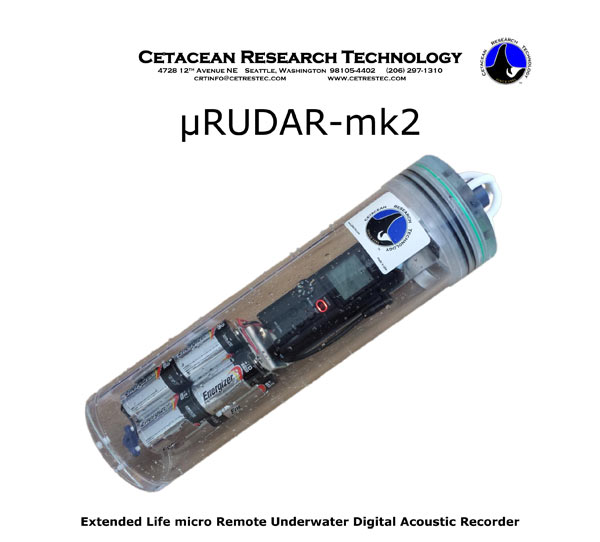
\includegraphics[width=0.70\textwidth]{graphics/uRUDAR-mk2.jpg}
    \caption{uRUDAR-mk2 fixed monitoring device\cite{computing_microrudar_nodate}}
    \label{fig:uRUDAR}
\end{figure}

\subsubsection{RUDAR (Remoter Underwater Digital Acoustic Recorder)}
Another recording device from Cetacean research technology is the RUDAR (Remoter Underwater Digital Acoustic Recorder), seen in \textit{Figure~\ref{fig:Rudar}}. 
It is a autonomous recording device that is small enough to be hand deployed from a small boat.
The recording system uses the ST400 mobile data recorder and sound level monitor. 
The system has a working depth of 1.5-3.5km it is able to record from 4 hydrophones at 24-bit resolution.
The data is written to an internal hard drives and is able to record 2 independent schemes and sample rates at the same time \cite{cetacean_research_technology_rudar_2021}.

\begin{figure}[h]
    \centering
    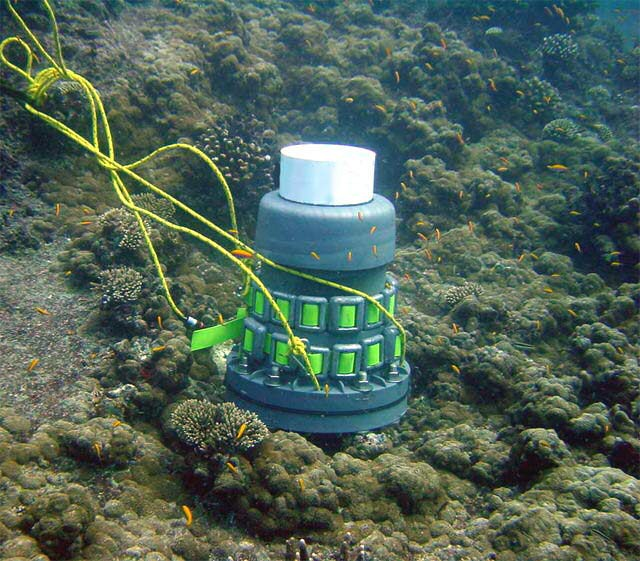
\includegraphics[width=0.70\textwidth]{graphics/Rudar.jpg}
    \caption{RUDAR recording device \cite{cetacean_research_technology_rudar_2021}}
    \label{fig:Rudar}
\end{figure}

%\fxfatal{TALA KANSKI UM F-pod hér \cite{noauthor_f-pod_nodate}}

\subsubsection{Persistent near real‐time passive acoustic monitoring for baleen whales from a moored buoy.}
A system has been developed for the United States Coast Guard that is capable of long term remote deployment. 
The system consist of a moored buoy that can provide data collection and transmission.
It has passive acoustic instruments such as digital acoustic monitoring(DMON) and a low-frequency detection and classification(LFDCS) firmware.
The system has three hydrophones and a a programmable Texas Instruments TMS320C55 digital signal processor (DPS) as well as GPS.
The firmware is used to build a spectogram of the recorded sounds when the mooring is recovered.
An example of which can be seen \textit{Figure \ref{fig:SpectoExamp}}.
It then classifies the sound calls by comparing attributes of the pitch track to known call types. 
The mooring hardware of the surface buoy is used for power delivery as well as data transmission. 
The system has an internal battery capacity of 450 Ah. 
%The audio is recorded with a sample frequency of 2kHz. 
It is designed to operate for a period of 1 year at a time has a maximum data transfer rate of 8Kb per hour through Iridium global communication system \cite{baumgartner_persistent_2019}.

\begin{figure}[h]
    \centering
    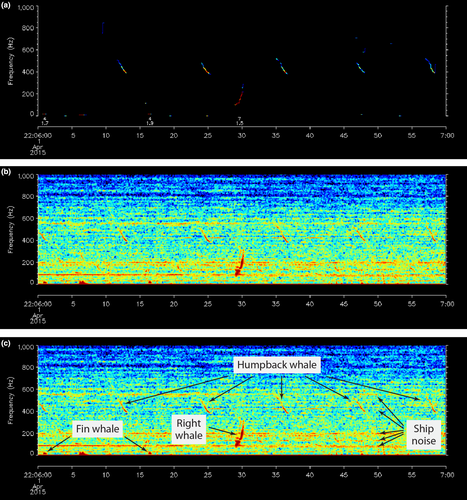
\includegraphics[width=0.60\textwidth]{graphics/spectogram.png}
    \caption{Spectogram that can be produced once the mooring is recovered.
    (a) In near-real time detection information (b) spectogram for a the given time period seen in (a) at 2000Hz sampling rate (c) addition of annottations of sound source to spectogram seen in (b)\cite{baumgartner_persistent_2019}}
    \label{fig:SpectoExamp}
\end{figure}

The setup of the of the system can be seen in \textit{Figure~\ref{fig:DMON/LFDCS}} from the moored surface buoy at the top, to the monitoring device at the bottom of the ocean.

\begin{figure}[h]
    \centering
    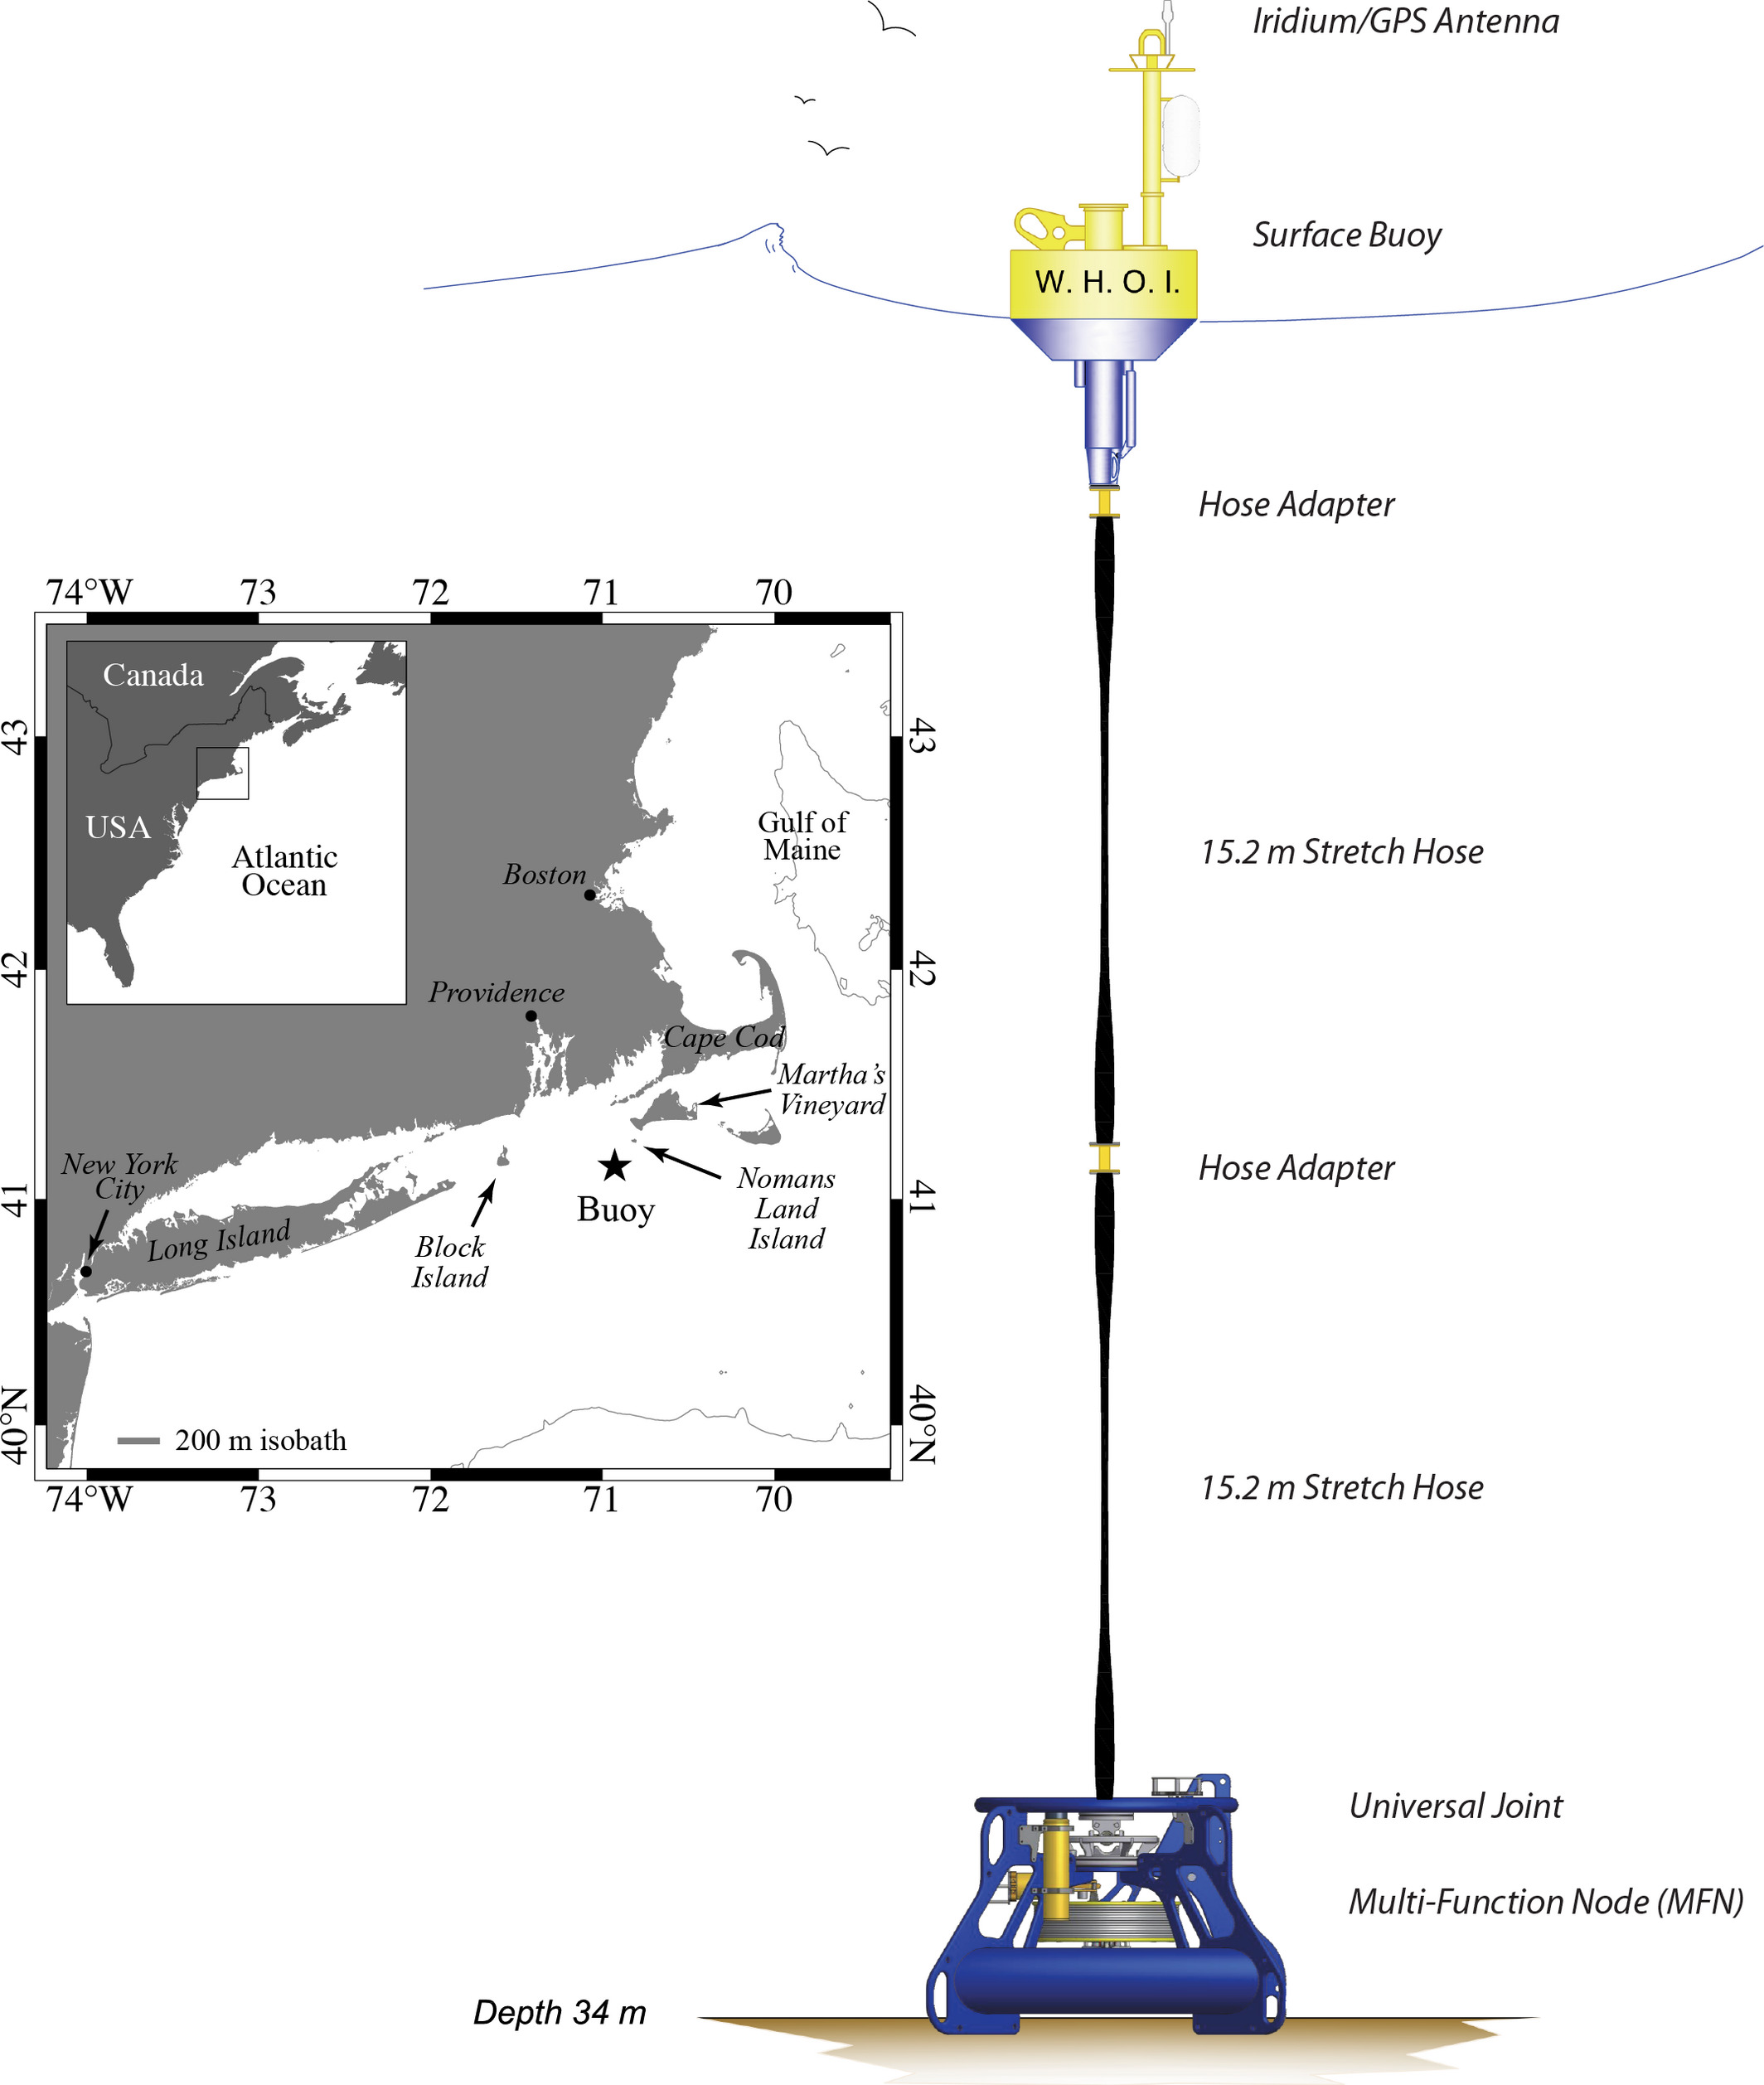
\includegraphics[width=0.70\textwidth]{graphics/DMONbuoy.jpg}
    \caption{A moored buoy using DMON/LFDCS systems, designed for 1 year deployments\cite{baumgartner_persistent_2019}}
    \label{fig:DMON/LFDCS}
\end{figure}




%%% Local Variables: 
%%% mode: latex
%%% TeX-master: "DEGREE-NAME-YEAR"
%%% End: 
